\documentclass{standalone}

\usepackage{tikz}
\usetikzlibrary {arrows.meta}

\begin{document}

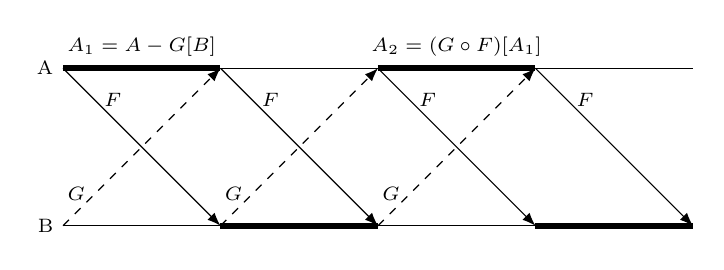
\begin{tikzpicture}[every node/.style={font=\scriptsize}]

  % Define points A and B as horizontal lines
  \node[left] (A) at (0,2) {A};
  \draw (0,2) -- (8,2);
  \node[left] (B) at (0,0) {B};
  \draw (0,0) -- (8,0);

  % Define A0 and A1 as segments on line A
  \draw[line width=2pt] (0,2) -- (2,2) node[midway,above] {$A_1 = A - G[B]$};
  \draw[line width=2pt] (4,2) -- (6,2) node[midway,above] {$A_2 = (G \circ F)[A_1]$};

  \draw[line width=2pt] (2,0) -- (4,0);
  \draw[line width=2pt] (6,0) -- (8,0);

  % Draw arrows and label them
  \draw[-{Latex[fill=black]},dashed] (0,0) -- (2,2) node[pos = 0.2, left] {$G$};
  \draw[-{Latex[fill=black]}] (0,2) -- (2,0) node[pos = 0.2, right] {$F$};
  \draw[-{Latex[fill=black]}] (2,2) -- (4,0) node[pos = 0.2, right] {$F$};

  \draw[-{Latex[fill=black]},dashed] (2,0) -- (4,2) node[pos = 0.2, left] {$G$};
  \draw[-{Latex[fill=black]}] (4,2) -- (6,0) node[pos = 0.2, right] {$F$};
  \draw[-{Latex[fill=black]}] (6,2) -- (8,0) node[pos = 0.2, right] {$F$};

  \draw[-{Latex[fill=black]},dashed] (4,0) -- (6,2) node[pos = 0.2, left] {$G$};

\end{tikzpicture}

\end{document}